\section{Evoluzione collisionale}\linkdest{collisions}

\subsection{Erosione, craterizzazione, rottura catastrofica}

\begin{frame}{Effetti degli urti}
\begin{columns}[T] \begin{column}{0.7\textwidth}
\begin{block}{Shattering/Dispersion: ri-accumulazione}
\begin{itemize}\item Energia d'impatto per unit\'a di massa del bersaglio perch\'e si abbia rottura catastrofica. \item Distribuzione iniziale dei frammenti (shattering) \item Composizione bersaglio e rotazione\end{itemize}
\begin{equation*}f_1=\frac{\text{m greater fragment}}{M_b}\end{equation*}
Strenght: Minimo sforzo per rottura.
\end{block}
\end{column}\begin{column}{0.3\textwidth}
\begin{block}{Velocit\'a relativa}\begin{itemize}\item Sistema solare interno: $\SI{10}{\kilo\meter\per\second}$\item Pianeti giganti/asteroidi/TNO: $\si{\kilo\meter\per\second}$\end{itemize}
\end{block}
\end{column}\end{columns}
\begin{itemize}\item Erosione \item Craterizzazione \item Rottura catastrofica
\end{itemize}
\end{frame}

\begin{wordonframe}{Effetti degli urti}
\begin{block}{Velocit\'a di fuga}
$v_e=\sqrt{\frac{2GM}{r}}=r\sqrt{\frac{8\pi G\rho}{3}}$, per $\rho\approx\SI{2}{\gram\per\cubic\cm}$: $v_e(\si{\meter\per\second})=r(\si{\kilo\meter})$
\end{block}
\begin{block}{Strenght}
Strenght: Minimo sforzo (Forza/superficie o energia/volume) per rottura (per compressione/tensione, impatto).
\end{block}
\begin{block}{Bersglio di basalto}
Basalto: $S\approx\SI{e7}{\erg\per\cubic\cm}$, $v_r=\SI{5}{\kilo\meter\per\second}$, $\frac{M_b}{M_p}\approx\num{e-4}$.
\end{block}
Fujiwara ('70): $f_1=0.5(\frac{SM}{\rho E/2})^{1.24}$.
Corpi soggetti a pressione hanno strength maggiore.
\end{wordonframe}

\begin{frame}{Distribuzione dei frammenti}
Collisioni a velocit\'a subsonica producono frammentazioni diverse
\begin{columns}[T]\begin{column}{0.5\textwidth}
\begin{block}{Massa}
$N(>m)\propto m\expy{-q},\ q\approx0.8$
\end{block}
\end{column}\begin{column}{0.5\textwidth}
\begin{block}{Velocit\'a}
$f(>v)\propto(\frac{v}{v_0})\expy{-k}$
\end{block}
\end{column}  \end{columns}
$F_{ke}=\frac{E_{ke}}{E_{imp}}$ cresce con energia specifica d'impatto secondo legge di potenza.
\end{frame}

\begin{frame}{Famiglie asteroidali}
\begin{block}{Limiti su S e $F_{ke}$ da osservazioni di asteroidi}
Asteroidi ($>\SI{150}{\meter}$) hanno $\tau_{spin}>\SI{2}{\hour}$: rubber piles (riaccumulazione: limite fissione, basso S,$F_{ke}$).
\end{block}
\begin{block}{Effetti delle collisioni su asteroidi ($R>\SI{100}{\kilo\meter}$)}
\begin{itemize}\item Famiglie dinamiche \item Asteroidi doppi \item LASPA: asteroidi di forma allungata (LA) e velocemente rotanti\end{itemize}
\end{block}
\end{frame}

\begin{wordonframe}{Risultanze di collisioni su asteroidi}
\begin{block}{LASPA: Ellissoidi triassiali di Jacobi.}
Urto che trasferisce grande momento angolare e frattura il corpo: $F_{ke}<\frac{2v_e}{v_i}$
\end{block}
\end{wordonframe}

\subsection{Deformazioni}

\begin{frame}{Deformazioni}
\begin{block}{Strain tensor}
\begin{align*}
&\epsilon_{ik}=\frac{1}{2}[\PDy{x_k}{\epsilon_i}+\PDy{x_i}{\epsilon_k}+(\PDy{x_i}{\epsilon_l}\PDy{x_k}{\epsilon_l})]:\ dV'=dV[1+\Tr{\epsilon}]
\end{align*}
\end{block}
\begin{block}{Stress tensor e equilibrio idrostatico}
\begin{columns}[T]\begin{column}{0.5\textwidth}
Forza per unit\'a di volume: $F_i=\PDy{x_k}{\sigma_{ik}}$.
\end{column} \begin{column}{0.5\textwidth}
Equilibrio idrostatico: $\PDy{x_k}{\sigma_{ik}}+\rho g_i=0$.
\end{column}  \end{columns}
Compressione uniforme: $\epsilon_{ik}=-\frac{P}{3K}\delta_{ik}$.
\end{block}
\begin{block}{Lavoro fatto a seguito delle deformazioni}
\begin{columns}[T]\begin{column}{0.5\textwidth}
\begin{align*}
&\int\delta W\,dV=\int\PDy{x_k}{\sigma_{ik}}\delta\epsilon_i\,dV\\
&\approx-\int\sigma_{ik}\delta\epsilon_{ik}\,dV
\end{align*}
\end{column}\begin{column}{0.5\textwidth}
\begin{align*}
&\sigma_{ik}=\Dcvar{\PDy{\epsilon_{ik}}{E}}{}=\Dcvar{\PDy{\epsilon_{ik}}{F}}{T}
\end{align*}
Materiale amorfo e isotropo:
$F=F_0+\mu(\epsilon_{ij}-\frac{1}{3}\delta_{ik}\epsilon_{ll})^2+\frac{K}{2}\epsilon_{ll}^2$
\end{column}\end{columns}
\end{block}
\end{frame}

\begin{wordonframe}{Strain, stress, thermodynamical quantities}
$[\sigma]=[S]=[P]=$Forza/superficie=Energia/Volume.
\begin{align*}
&dE=TdS+\sigma_{ik}\,d\epsilon_{ik}\\
&dF=-SdT+\sigma_{ik}\,d\epsilon_{ik}
\end{align*}
Piccole deformazioni: $F=F_0+\frac{\lambda_{iklm}}{2}\epsilon_{ik}\epsilon_{lm}$. In solido amorfo lo sviluppo in serie contiene scalari: $F=F_0+\frac{\lambda}{2}\epsilon_{ii}^2+\mu\epsilon_{ik}\epsilon_{ik}$.
K modulo compressione, $\mu$ deformazione di taglio ($\lambda$, $\mu$ coefficienti di Lam\'e).
$\Tr{\epsilon}=-\frac{P}{K}$.
\end{wordonframe}

\begin{frame}{Onde nei solidi}
\begin{columns}[T]\begin{column}{0.6\textwidth}
\begin{block}{Legge di Hooke}
\begin{equation*}
\sigma_{ik}=K\delta_{ik}\epsilon_{ll}+2\mu(\epsilon_{ik}-\frac{1}{3}\delta_{ik}\epsilon_{ll})
\end{equation*}
\end{block}
\begin{block}{Onde elastiche}
\begin{align*}
&\rho\ddvec{\epsilon}=[K+\frac{1}{3}\mu]\nabla(\scap{\nabla}{\epsilon})+\mu\nabla^2\vec{\epsilon}\\
&\PtwoDy{t}{\vec{\epsilon}_l}-c_l^2\nabla^2\vec{\epsilon}_l=0,\ c_l=\sqrt{\frac{K+4/3\mu}{\rho}}\\
&\PtwoDy{t}{\vec{\epsilon}_T}-c_T^2\nabla^2\vec{\epsilon}_T=0,\ c_T=\sqrt{\frac{\mu}{\rho}}
\end{align*}
\end{block}
\end{column} \begin{column}{0.4\textwidth}
\begin{block}{Onde longitudinali (unidirezionale)}
\begin{align*}
&\sigma_l=-\rho u_lc_l\\
&\sigma_T=\frac{\nu}{1-\nu}\sigma_l
\end{align*}
$\nu$ Poisson's ratio.
\end{block}
\end{column}  \end{columns}
\end{frame}

\begin{wordonframe}{Onde nei solidi}
\begin{align*}
&\epsilon_{ik}=\frac{1}{9K}\delta_{ik}\sigma_{ll}+\frac{1}{2\mu}(\sigma_{ik}-\frac{1}{3}\delta_{ik}\sigma_{ll})\\
&[K+\frac{1}{3}\mu]\nabla(\scap{\nabla}{\epsilon})+\mu\nabla^2\vec{\epsilon}=0
\end{align*}
\begin{columns}[T]\begin{column}{0.4\textwidth}\begin{block}{Intensit\'a}
\end{block}
\end{column} \begin{column}{0.6\textwidth}
\begin{block}{Stress onde longitudinali/trasversali}
\end{block}
\end{column}  \end{columns}
\end{wordonframe}

\begin{frame}{Hugoniot elastic limit}
\begin{columns}[T]\begin{column}{0.7\textwidth}
\begin{figure}[!ht]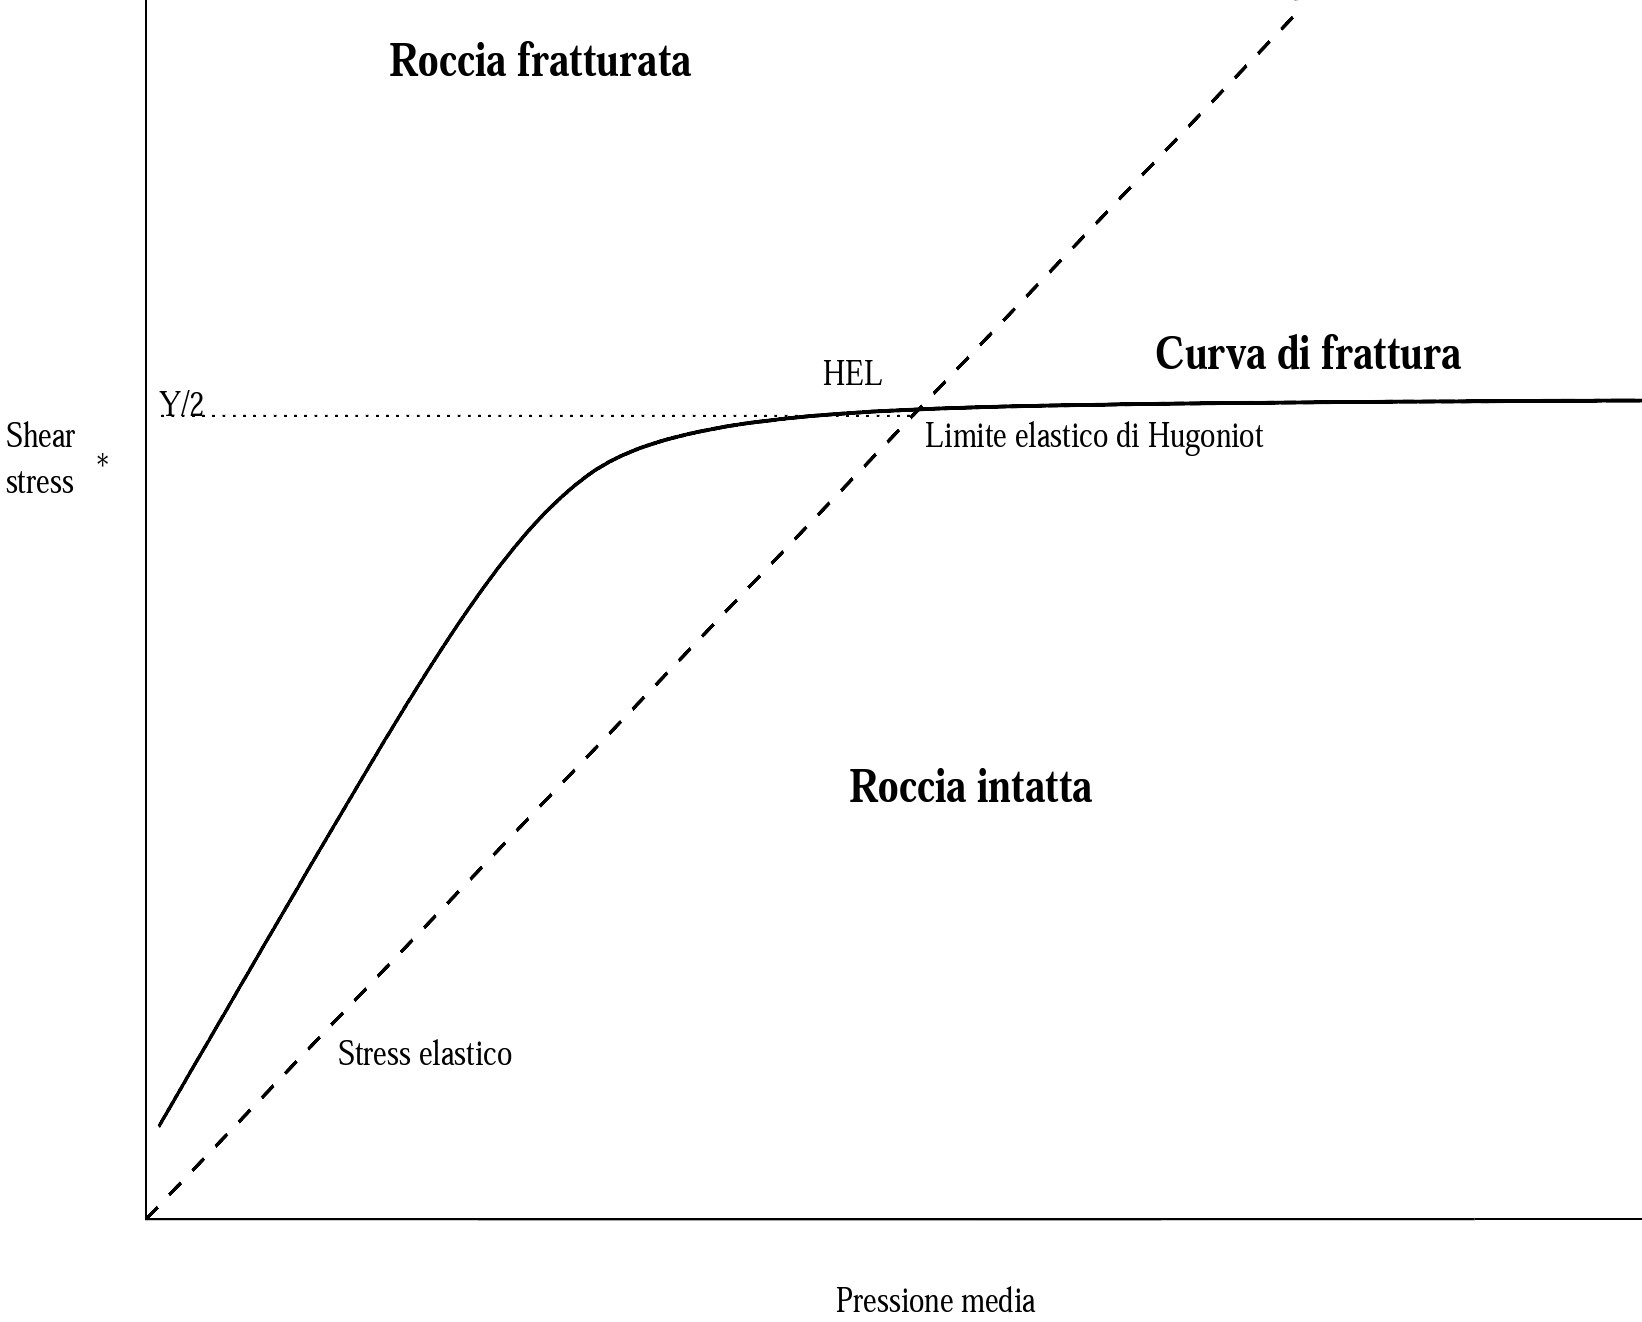
\includegraphics[keepaspectratio,width=0.9\textwidth]{shearstress}\end{figure}
\end{column} \begin{column}{0.3\textwidth}
\tikz\draw[->] (0,0) node[right] {Elastiche}--(0,1) node[right] {Onde d'Urto} node[midway,right] {Plastiche};
\begin{block}{Regime elastico}$|\sigma_l-\sigma_T|<Y$, Y yield stress.\end{block}
\end{column}  \end{columns}
\end{frame}

\begin{wordonframe}{HEL}
Suoerato il limite di Hugoniot si ha precursore elastico che si propaga con velocit\'a $c_l$ e onda plastica che si propaga con velocit\'a $c_b$: per $c_b>c_l$ si hanno onde d'urto.
\end{wordonframe}

\subsection{Teoria del danno}

\begin{frame}{Rottura}
\begin{block}{Distribuzione di Weibull}
Numero difetti attivi per deformazione $\epsilon$:
\begin{equation*}
N(\epsilon)=K\epsilon^m
\end{equation*}
$m$(materiale), $K\propto V$
\end{block}
Per rottura di corpi grandi in seguito a impatti ad alta velocit\'a siamo in regime di strength dinamica.
\begin{block}{Strain rate}
Vicino al punto d'impatto $\dot{\epsilon}\approx\frac{v_P}{l_P}$.
\end{block}
\end{frame}

\begin{wordonframe}{Teori del danno}
\begin{block}{difetti in seguito a urti}
Le onde dovute all'impatto attraversano il corpo e attivano processi di rottura; difetti crescono fino a dar vita a fratture macroscopiche.
\end{block}
\begin{block}{Transizione regime strength statica/dinamica}
Minima deformazione per rottura: $\epsilon_{min}\propto(K_0R^3)\expy{-\frac{1}{m}}$.
Strength tensile: $\propto\dot{\epsilon}\expy{\frac{3}{m+3}}\propto l_P\expy{-\frac{1}{4}}$.
\end{block}
\end{wordonframe}

\begin{frame}{Timing nei processi di urto}
\begin{itemize}
\item Allocazione energia d'impatto: estesa fratturazione
\item Espulsione frammenti a bassa velocit\'a: basso S basso $F_{ke}$. (Estesa fratturazione: strength/energy transfer bassa.)
\end{itemize}
\end{frame}

\begin{frame}{Modello di Grady-Kipp}
\begin{block}{Parametro di danneggiamento}
\begin{equation*}
\sigma_{ij}=K(1-D)\epsilon_{ll}\delta_{ij}+2\mu(1-D)(\epsilon_{ij}-\frac{1}{3}\epsilon_{ll}\delta_{ij})
\end{equation*}
\end{block}
\begin{block}{Fratture per unit\'a di volume $n$: $D=nV_f$}
\end{block}
\begin{block}{Evoluzione del danno nel tempo}
Le fratture crescono con velocit\'a $c_g$, $V_f=\frac{4}{3}\pi c_g^3t^3$:
\begin{equation*}D(t)=\int_{-\infty}^t\dot{n}(t')V(t-t')\,dt'=\frac{4}{3}\pi c_g^3\int_{-\infty}^t\TDy{\epsilon}{N}\dot{\epsilon}(1-D)(t-t')^3\end{equation*}
\end{block}
\begin{block}{Distribuzione dimensione frammenti}
\begin{equation*}
F(L)=\frac{\pi mK_0L^3}{12c_g}(t_f-\frac{L}{2c_g})\expy{m-1}\dot{\epsilon}^m
\end{equation*}
\end{block}
\end{frame}

\begin{wordonframe}{Grady-Kipp}
$t_f$ tempo a cui il danno \'e completo.
\end{wordonframe}

